\documentclass[journal]{IEEEtran}

% =========================
% Packages
% =========================
\usepackage{amsmath,amssymb,amsthm}
\usepackage{graphicx}
\usepackage[utf8]{inputenc}
\usepackage[T1]{fontenc}
\newtheorem{assumption}{Assumption}
\usepackage{cite}
\usepackage{booktabs}
\usepackage{algorithmic}
\usepackage{array}
\usepackage{url}
\usepackage{hyperref}
\usepackage{xcolor}
\usepackage{booktabs}
\usepackage{amssymb}
\usepackage{tikz}
\usetikzlibrary{arrows.meta,positioning}
% =========================
% Theorem Environments
% =========================
\newtheorem{theorem}{Theorem}
\newtheorem{lemma}{Lemma}
\newtheorem{proposition}{Proposition}
\newtheorem{corollary}{Corollary}
\newtheorem{definition}{Definition}
\newtheorem{remark}{Remark}

% =========================
% Title
% =========================
\title{The Geometry of Adversarial Identity Cost:
	Structural Limits of Sybil Resistance in Open Systems}

\author{Anonymous Author(s)}

\begin{document}
	
	\maketitle
	
	% =========================
	% Abstract
	% =========================
	
	\begin{abstract}
		
		Open and permissionless systems mitigate Sybil attacks by
		binding influence to scarce resources.
		However, \emph{aggregate scarcity alone does not determine how
			the cost of sustaining multiple identities scales over time}.
		Many widely deployed resources---such as computation and financial
		capital---are \emph{divisible and reusable}: they can be
		subdivided, transferred, and reapplied across identities
		and time without proportional marginal expenditure.
		As a result, adversarial effort may be amortized across identities,
		enabling large-scale identity replication at sublinear cost.
		
		This paper develops an axiomatic framework for analyzing
		security-weighting resources through the lens of
		\emph{adversarial cost geometry}.
		We identify a small set of resource properties---including
		divisibility, additivity of influence, temporal reusability,
		identity transferability, and throughput boundedness---that
		characterize the asymptotic growth of sustained adversarial cost.
		
		Under a standard amortized coordination model,
		we establish an asymptotic boundary between two resource classes.
		Within the present abstraction, mechanisms grounded in
		divisible, reusable resources admit identity amortization,
		yielding $C(s,T)=o(sT)$;
		the marginal cost per additional identity does not grow
		with the time horizon.
		In contrast, throughput-bounded, non-transferable,
		window-local resources indicate a linear scaling regime,
		$C(s,T)=\Omega(sT)$, with marginal cost $\Delta(s,T)=\Omega(T)$.
		
		Under the assumptions considered here, protocol rules that
		redistribute a fully divisible and reusable resource
		may be insufficient to enforce linear per-identity cost.
		The framework is intended as a resource-centric asymptotic lens
		that complements existing deployment-level and protocol-level
		analyses rather than replacing them.
		We accompany the theoretical results with analytical illustrations
		of the scaling regimes across varying identity counts,
		time horizons, and coordination overhead models.
		
	\end{abstract}
	
	
	\begin{IEEEkeywords}
		Sybil attacks, adversarial cost models, distributed security,
		resource parallelizability, identity scaling.
	\end{IEEEkeywords}
	% ============================================================
	\section{Introduction}
	
	\subsection{Motivation}
	
	Open and permissionless systems must regulate influence under adversarial
	conditions in which identity creation is inexpensive and effectively
	unbounded.
	The classical formulation of this problem is the Sybil
	attack~\cite{douceur2002sybil}, where a single adversarial entity
	generates multiple identities to amplify control over a distributed system.
	This vulnerability affects peer-to-peer overlays, blockchain
	consensus~\cite{lamport1982byzantine,fischer1985flp,castro1999pbft,garay2015backbone,ren2019nakamoto},
	decentralized governance, reputation systems,
	and distributed access-control
	frameworks~\cite{bonneau2015sok,narayanan2016bitcoinbook,gencer2018decentralization,decker2013information}.
	
	A dominant design paradigm mitigates Sybil attacks by binding influence
	to the possession or expenditure of a scarce resource.
	Proof-of-Work (PoW) associates block-production probability with
	computational effort~\cite{garay2015backbone},
	while Proof-of-Stake (PoS) binds influence to locked financial capital
	\cite{kiayias2017ouroboros}.
	Such mechanisms have been analyzed under partially synchronous network
	models, yielding safety and liveness guarantees in terms of aggregate
	adversarial resource
	ownership~\cite{dwork1988partial,garay2015backbone,kiayias2017ouroboros}.
	
	However, many security-critical operations in open systems function at
	the \emph{identity layer} rather than the resource layer.
	Examples include decentralized governance~\cite{buterin2014dao},
	committee selection~\cite{gilad2017algorand},
	reputation systems~\cite{resnick2000reputation},
	rate-limited participation~\cite{li2017sybilcontrol},
	and identity-based access control.
	In these settings, the relevant security question shifts from how much
	resource an adversary controls in aggregate to how the cost of
	\emph{sustaining multiple identities} scales with their number and the
	duration of participation.
	
	\medskip
	\noindent
	\textbf{A Resource-Structural Perspective.}
	A frequently implicit property of widely deployed resources is that
	they are \emph{divisible and reusable}: computational capacity and
	financial capital can be subdivided, delegated, and reapplied across
	identities without proportional marginal expenditure.
	Mining pools in PoW and stake delegation in PoS illustrate this---once
	aggregate resource ownership is acquired, it can be redistributed across
	arbitrarily many identities while preserving total
	influence~\cite{rosenfeld2011analysis,gencer2018decentralization,
		kiayias2017ouroboros,saleh2021blockchain}.
	As a result, adversarial effort may be \emph{amortized across
		identities}: a single adversary can sustain many identities while
	incurring only slowly growing marginal cost.
	
	This observation reveals an asymptotic limitation of scarcity-based
	defenses not captured by existing analyses.
	Economic models focus on equilibrium cost-of-corruption
	\cite{budish2018economic,budish2024economic},
	while protocol-level analyses focus on aggregate adversarial
	influence~\cite{miller2016honeybadger,sompolinsky2015ghost}.
	Neither framework isolates the resource properties that govern how
	adversarial cost scales with the number of sustained identities.
	
	This motivates the following question:
	
	\begin{quote}
		\emph{What properties must a security resource possess
			for sustained adversarial cost to grow proportionally
			with the number of active identities?}
	\end{quote}
	
	\subsection{Contribution and Framing}
	
	This paper develops a resource-centric asymptotic lens for analyzing
	identity-level Sybil resistance.
	The objective is not to replace deployment-specific or protocol-level
	security analyses, but to isolate how the structural properties of a
	security-weighting resource determine the asymptotic geometry of
	adversarial identity cost.
	The framework is intended to complement existing analyses---including
	aggregate-resource consensus models and economic equilibrium
	analyses---by identifying when divisibility and reusability enable
	adversarial cost amortization.
	
	Under a standard amortized coordination model,
	we establish an asymptotic boundary between two resource classes:
	
	\begin{itemize}
		\item Resources satisfying \emph{divisibility, additivity,
			transferability, and temporal reuse}
		admit identity amortization within the considered model,
		yielding $C(s,T) = o(sT)$.
		
		\item Resources that are \emph{rate-limited}, non-transferable,
		and window-local indicate the scaling regime
		$C(s,T) = \Omega(sT)$.
	\end{itemize}
	
	Within the considered model, this boundary reflects the resource class
	of the underlying mechanism rather than its protocol-level design.
	Fully divisible and reusable resources admit sublinear per-identity
	cost regardless of the protocol rules designed around them, within the present abstraction.
	Rate-limited, non-transferable resources, by contrast, impose
	per-identity participation constraints that resist amortization.
	
	As a secondary implication, divisibility and reusability induce
	\emph{centralization pressure}: because resource aggregation does not
	incur proportional identity-level cost, participants are incentivized
	to pool or delegate, consistent with empirically observed behavior in
	mining pools and delegation markets~\cite{bonneau2015sok,bano2019consensus}.
	
	\subsection{Contributions}
	
	\begin{itemize}
		
		\item \textbf{Axiomatic Resource Framework.}
		We introduce a framework based on properties including
		divisibility, additivity of influence, temporal reusability,
		identity transferability, and throughput boundedness.
		
		\item \textbf{Asymptotic Limit for Divisible Resources.}
		We establish that mechanisms grounded in fully divisible,
		reusable resources admit identity amortization within the
		considered model, yielding $C(s,T)=o(sT)$.
		
		\item \textbf{Linear Lower Bound for Rate-Limited Resources.}
		We establish that throughput-bounded, non-transferable resources
		imply $C(s,T)=\Omega(sT)$.
		
		\item \textbf{Asymptotic Scaling Separation.}
		We establish that the two resource classes induce
		asymptotically disjoint cost regimes under the boundary
		conditions characterized in this work.
		
		\item \textbf{Design Implications.}
		Under the considered model, identity-level cost scaling is
		constrained by resource structure rather than protocol syntax.
		
	\end{itemize}
	
	\subsection{Organization of the Paper}
	
	Section~II reviews related work.
	Section~III introduces the system model.
	Section~IV formalizes the axiomatic framework.
	Sections~V and VI establish the main bounds.
	Section~VII proves the scaling separation theorem.
	Section~VIII presents concrete resource instantiations.
	Sections~IX and X discuss implications and limitations.
	Section~XI presents analytical illustrations of the scaling regimes.
	% ============================================================
	\section{Related Work}
	
	Prior research has addressed adversarial influence and Sybil attacks
	in open systems from several perspectives.
	However, these research directions typically study security questions
	that differ from the one considered in this paper.
	In particular, existing work largely focuses on
	identity admission, consensus safety, or economic incentives,
	while the present work studies how the
	\emph{structural properties of security resources determine
		the asymptotic cost of sustaining multiple identities over time}.
	
	Table~\ref{tab:related_positioning} summarizes the distinction
	between major research directions and the focus of this paper.
	
	\begin{table*}[t]
		\centering
		\caption{Positioning of This Work Relative to Prior Literature}
		\label{tab:related_positioning}
		
		\begin{tabular}{p{3.2cm}p{4.6cm}p{5.2cm}}
			\toprule
			\textbf{Research Line} & \textbf{Primary Security Question} & \textbf{Representative Works} \\
			\midrule
			
			Sybil Attack Literature &
			Can adversaries create multiple identities, and how can identity
			creation be restricted or detected? &
			\cite{douceur2002sybil,yu2006sybilguard,yu2008sybillimit,danezis2009sybilinfer,wang2019attack,lesniewski2020analysis} \\
			
			Blockchain Consensus Security &
			Under what conditions does aggregate adversarial resource ownership
			violate safety or liveness properties of consensus protocols? &
			\cite{garay2015backbone,ren2019nakamoto,pass2017hybrid,kiayias2017ouroboros,pass2017fruitchains,eyal2018bitcoinng} \\
			
			Economic Analyses of Consensus &
			What equilibrium incentives and corruption costs arise in
			resource-weighted consensus systems? &
			\cite{budish2018economic,budish2024economic,kroll2013economics,rosenfeld2014analysis,tramer2020slush}\\
			
			Identity-Binding Mechanisms &
			How can systems enforce one-person--one-identity mappings
			through ceremonies or identity verification? &
			\cite{borge2017pop,ford2020pseudonym} \\
			
			\textbf{This Paper} &
			\textbf{How do structural properties of security resources determine
				the asymptotic cost of sustaining multiple identities over time?} &
			Structural analysis of identity-scaling cost \\
			
			\bottomrule
		\end{tabular}
	\end{table*}
	
	\subsection{Resource-Based Sybil Defenses}
	
	The Sybil attack, formally introduced by Douceur \cite{douceur2002sybil},
	established that identity replication in open systems
	cannot be prevented without binding influence to scarce resources.
	Modern permissionless systems implement this principle
	through resource-weighted mechanisms.
	
	Nakamoto’s proposal \cite{nakamoto2008bitcoin}
	introduced Proof-of-Work (PoW), in which block-production
	probability scales with computational effort.
	Subsequent formal analyses
	\cite{garay2015backbone,ren2019nakamoto,pass2017hybrid,pass2017fruitchains}
	established security properties of Nakamoto-style consensus,
	including chain growth, common prefix, and chain quality guarantees.
	
	Proof-of-Stake (PoS) systems replace computational effort
	with locked financial capital.
	Protocols such as Ouroboros \cite{kiayias2017ouroboros}
	and its extensions
	\cite{kiayias2018ouroboros,kiayias2020genesis}
	provide provable security guarantees under partially synchronous
	network models, while protocols such as Algorand
	\cite{gilad2017algorand,gilad2017algorand_extended}
	use cryptographic sortition to sample committees
	proportionally to stake.
	
	Empirical and systems-level analyses further study the
	security and performance of blockchain consensus mechanisms.
	Work on mining incentives, pooling behavior, and adversarial strategies
	\cite{eyal2014majority,gervais2016security,rosenfeld2014analysis,tramer2020slush}
	demonstrates how adversarial resources are frequently aggregated,
	pooled, and redistributed across multiple logical identities.
	Other studies analyze decentralization and deployment realities
	\cite{bonneau2015sok,gencer2018decentralization,gervais2014isbitcoin,alwen2019blockchain}.
	
	Additional work studies network-level adversaries such as
	eclipse and routing attacks
	\cite{heilman2015eclipse,apostolaki2017hijacking,neudecker2019network},
	as well as economic stability of mining rewards and fee mechanisms
	\cite{carlsten2016instability,kroll2013economics,budish2018economic,budish2024economic}.
	
	Despite this extensive literature,
	these analyses consistently reason about
	\emph{aggregate adversarial resource share}.
	Security guarantees are expressed in terms of the
	fraction of computational power or stake controlled by
	an adversary.
	However, these models do not explicitly analyze how
	adversarial cost scales with the number of sustained identities.
	
	
	\subsection{Graph-Based and Social-Structure Defenses}
	
	Another line of work constrains Sybil proliferation
	using the structure of social networks.
	Mechanisms such as SybilGuard \cite{yu2006sybilguard}
	and SybilLimit \cite{yu2008sybillimit}
	exploit the limited number of attack edges between
	honest and adversarial regions of a social graph
	to restrict the influence of Sybil identities.
	
	Later work such as SybilInfer \cite{danezis2009sybilinfer}
	applies probabilistic inference over trust graphs to detect
	clusters of suspicious nodes.
	These approaches can significantly increase the difficulty
	of creating large Sybil regions when the social graph
	exhibits strong connectivity properties.
	
	However, their guarantees depend heavily on the topology
	and trust assumptions of the underlying network.
	When such assumptions fail,
	these mechanisms do not provide explicit bounds on
	how adversarial cost scales with the number of sustained identities.
	More generally, these approaches constrain the \emph{placement}
	of identities within a social graph, but do not characterize
	the \emph{cost of sustaining identities} as their number grows.
	\subsection{Randomness and Committee Sampling}
	
	Leader election and committee sampling mechanisms
	often rely on cryptographic randomness primitives.
	Verifiable random functions (VRFs) \cite{micali1999vrf}
	enable unpredictable leader selection,
	while bias-resistant randomness protocols
	\cite{syta2017scalable}
	enable robust distributed randomness generation.
	
	Composable analyses of blockchain protocols
	\cite{garay2015backbone,pass2017hybrid,pass2016snowwhite}
	demonstrate robustness under dynamic participation
	and partially synchronous networks.
	More recent asynchronous constructions such as
	HoneyBadgerBFT \cite{miller2016honeybadger}
	illustrate that scalable consensus can be achieved
	without strong synchrony assumptions.
	
	Nevertheless, these mechanisms continue to model
	adversarial capability in terms of aggregate resource ownership.
	Randomness primitives improve scalability and fairness
	of leader selection but do not alter the structural
	divisibility or transferability of the underlying resource.
	
	\subsection{Human-Centric Identity Mechanisms}
	
	Human-centric approaches attempt to enforce
	one-person--one-identity mappings through
	physical ceremonies, biometric verification,
	or behavioral signals.
	Proof-of-Personhood protocols \cite{borge2017pop}
	represent one prominent example,
	while later work explores pseudonym parties
	and social identity verification mechanisms
	\cite{ford2020pseudonym}.
	
	Such systems aim to restrict identity creation
	by binding credentials to real-world participants.
	However, these mechanisms primarily address
	identity admission rather than sustained participation.
	Once identities are admitted,
	influence may still be governed by reusable
	or transferable resources.
	
	Consequently, identity admission mechanisms alone
	do not guarantee linear adversarial cost over time.
	
	\subsection{Rate Limiting and Capability Systems}
	
	Systems research has long studied per-actor resource constraints.
	Capability-based security architectures
	\cite{levy1984capability}
	limit authority through unforgeable tokens,
	while congestion-control algorithms
	\cite{jacobson1988congestion}
	regulate per-flow network throughput.
	
	More recent hardware-based security architectures,
	including trusted execution environments such as
	Intel SGX \cite{costan2016intel},
	enable systems to bind computation to specific devices
	or execution contexts, enforcing hardware-rooted execution constraints.
	
	Such mechanisms impose intrinsic limits on per-identity or per-device
	throughput, effectively restricting the rate at which independent
	participants can generate verifiable activity.
	
	Although these frameworks effectively enforce
	per-actor or per-device rate limits,
	they are typically analyzed in terms of access control,
	network stability, or trusted hardware guarantees
	rather than adversarial identity scaling.
	
	\subsection{Positioning of This Work}
	This paper departs from prior research in two key ways.
	First, rather than analyzing specific protocols or admission
	mechanisms, we develop an axiomatic theory of
	\emph{security-weighting resources}.
	We formalize structural properties such as
	divisibility,
	additivity of influence,
	temporal reusability,
	identity transferability,
	and throughput boundedness,
	and analyze how these properties determine
	the geometry of adversarial cost.
	Second, we establish a structural separation at the extremal
	boundary conditions between resource classes.
	Parallelizable resources induce sublinear sustained identity
	cost within the present model,
	whereas throughput-bounded,
	non-transferable, window-local resources enforce
	\[
	C(s,T)=\Omega(sT).
	\]
	Unlike prior work on cost-of-corruption or equilibrium
	security~\cite{budish2018economic,budish2024economic}, our framework does not
	analyze the economic threshold required to corrupt a protocol
	instance. Instead, it studies how the structural properties of
	the underlying resource determine the asymptotic cost of
	sustaining multiple identities over time. Existing economic
	analyses characterize aggregate adversarial expenditure under
	equilibrium assumptions, while Sybil-defense
	mechanisms~\cite{li2017sybilcontrol} typically focus on
	identity admission or detection. In contrast, the present work
	isolates structural conditions under which adversarial identity
	cost becomes amortizable or remains proportional to the number
	of sustained identities---a dimension that neither aggregate
	cost models nor admission-based defenses address.
	Thus, unlike prior work that focuses on identity creation,
	consensus thresholds, or economic equilibria,
	our analysis identifies identity-level Sybil resistance
	as a consequence of the structural properties of the
	underlying resource class.
	Specifically, prior work does not isolate whether a fixed
	aggregate resource can be decomposed across many identities
	at sublinear marginal cost---the central question of this paper.
	% ============================================================
	\section{System Model}
	
	We consider an open and permissionless system in which identities
	are inexpensive to create and no trusted admission authority exists.
	Participation is therefore identity-unbounded,
	and adversaries may generate arbitrarily many identities
	at negligible syntactic cost.
	
	Security mechanisms regulate influence by binding participation
	to the possession or expenditure of a resource $R$.
	Our objective is to characterize how structural properties of $R$
	determine the scaling behavior of adversarial identity replication.
	
	\subsection{Notation}
	
	Table~\ref{tab:notation} summarizes the core notation used throughout the paper.
	
	\begin{table}[t]
		\centering
		\small
		\caption{Core Notation}
		\label{tab:notation}
		
		\begin{tabular}{ll}
			\toprule
			\textbf{Symbol} & \textbf{Meaning} \\
			\midrule
			$v$ & Identity (participant instance) \\
			$t$ & Time window index \\
			$T$ & Time horizon (number of windows) \\
			$s$ & Number of sustained identities \\
			$r_v(t)$ & Resource allocated to identity $v$ at time $t$ \\
			$W_v(t)$ & Influence of identity $v$ at time $t$ \\
			$f(\cdot)$ & Resource-to-influence mapping \\
			$S_t$ & Set of adversarial identities at time $t$ \\
			$C(s,T)$ & Cost to sustain $s$ identities over $T$ windows \\
			$\Delta(s,T)$ & Marginal identity cost \\
			\bottomrule
		\end{tabular}
		
	\end{table}
	
	\subsection{Open Identity Model}
	
	Let $\mathcal{U}$ denote the universe of potential participants.
	At each time window $t$, the system contains a set of active identities $V_t$.
	
	An adversary $\mathcal{A}$ is identity-unbounded:
	it may create, retire, and coordinate an arbitrary number of identities
	at negligible syntactic cost, consistent with the Sybil model~\cite{douceur2002sybil}.
	
	Let $S_t \subseteq V_t$ denote the subset of identities
	controlled by $\mathcal{A}$ during window $t$,
	with $|S_t| = s_t$.
	We impose no a priori bound on $s_t$.
	
	An identity is an abstract participant instance
	capable of receiving resource allocation and producing influence.
	
	\subsection{Time Model}
	
	Time is divided into discrete windows
	\[
	t = 1,2,\dots
	\]
	
	A window represents the minimal interval over which resource allocation
	and influence may be refreshed (e.g., block intervals or governance epochs).
	
	We evaluate security over a finite horizon of $T$ windows.
	An identity is said to be \emph{sustained} if it remains active
	throughout all windows $t = 1,\dots,T$.
	
	\subsection{Resource and Influence}
	Let $R$ denote the security-weighting resource.
	For each identity $v \in V_t$ and window $t$,
	\[
	r_v(t) \in \mathbb{R}_{\ge 0}
	\]
	denotes the allocated resource.
	Influence is determined by a mapping
	\[
	W_v(t) = f(r_v(t)).
	\]
	We do not impose structural assumptions on $f$ at this stage;
	these will be derived from properties of the resource $R$.
	
	\begin{definition}[Activation Threshold]
		There exists a constant $r_{\min} > 0$ such that
		an identity is active in window $t$ only if
		\[
		r_v(t) \ge r_{\min}.
		\]
	\end{definition}
	
	This captures the requirement that participation requires
	a strictly positive resource commitment.
	
	\begin{remark}
		The activation threshold $r_{\min}$ establishes a per-identity
		floor that any active identity must meet, regardless of resource
		structure.  This baseline cost is unavoidable and grows linearly
		with the number of sustained identities.  The structural
		separation established in Sections~V--VII does \emph{not} concern
		this baseline.  Rather, it asks whether a resource imposes an
		\emph{additional} per-identity, per-window cost beyond $r_{\min}$.
		Specifically, Theorem~1 shows that a fully parallelizable resource
		may not impose such additional cost within this model: an adversary need only acquire
		an aggregate allocation $r \ge s\,r_{\min}$ and redistribute it
		across $s$ identities, incurring no further $T$-scaling overhead.
		Theorem~2 shows that a throughput-bounded resource does impose this
		additional structure, making $r_{\min} \cdot T$ the unavoidable
		marginal cost per new identity.
	\end{remark}
	
	The total adversarial influence at time $t$ is
	\[
	W_{\mathcal{A}}(t) = \sum_{v \in S_t} W_v(t).
	\]
	
	\subsection{Adversarial Model}
	
	The adversary $\mathcal{A}$ is computationally unbounded
	but constrained by the structural properties of the resource $R$.
	
	Specifically, $\mathcal{A}$ may:
	
	\begin{itemize}
		\item Instantiate arbitrarily many identities.
		\item Allocate and redistribute resource across identities
		when permitted by the resource structure.
		\item Reuse or reallocate resource across time windows
		when temporal reuse is allowed.
		\item Coordinate identities without communication constraints.
	\end{itemize}
	
	This model subsumes aggregate-resource adversaries
	used in blockchain analyses~\cite{garay2015backbone,kiayias2017ouroboros},
	while remaining protocol-independent.
	
	\subsection{Model Scope and Coordination Assumptions}
	
	Our adversarial model assumes that identity coordination
	does not itself impose throughput constraints comparable to
	those enforced by the underlying security resource.
	
	In particular, we distinguish between:
	(i) resource-induced constraints, which arise from the
	structural properties of the security-weighting resource, and
	(ii) coordination overhead, which captures auxiliary costs
	associated with managing multiple identities.
	
	Throughout the paper, coordination costs are modeled
	separately through the function h(s,T), allowing the structural
	properties of the resource to be analyzed independently of
	implementation-specific orchestration mechanisms.
	
	The results established in Sections V--VII therefore isolate
	the scaling implications induced by resource structure rather
	than by assumptions about communication complexity,
	software architecture, or operational deployment details.
	
	\subsection{Adversarial Cost}
	
	We define the adversarial cost function $C(s,T)$
	as the minimum total resource expenditure required
	to sustain at least $s$ active identities
	over $T$ consecutive windows.
	
	To make the structure of costs precise, we decompose
	$C(s,T)$ into three components:
	\[
	C(s,T) = C_{\mathrm{stock}}(s) + C_{\mathrm{flow}}(s,T) + h(s,T),
	\]
	where:
	\begin{itemize}
		\item $C_{\mathrm{stock}}(s)$ is the one-time acquisition
		cost of resources that persist across all $T$ windows
		without renewal (e.g., staked capital, hardware);
		\item $C_{\mathrm{flow}}(s,T)$ is the cumulative
		per-window expenditure for resources that must be
		renewed each window (e.g., energy, device attestations,
		human participation);
		\item $h(s,T)$ is the coordination overhead of
		managing $s$ identities over $T$ windows.
	\end{itemize}
	
	Formally,
	\[
	C(s,T) =
	\inf
	\left\{
	\sum_{t=1}^{T} \mathcal{R}_{\mathcal{A}}(t)
	\;\middle|\;
	|S_t| \ge s \ \forall t \in \{1,\dots,T\}
	\right\}.
	\]
	
	The structural separation of Sections~V--VII concerns
	the scaling of $C_{\mathrm{flow}}(s,T)$:
	parallelizable resources admit $C_{\mathrm{flow}}(s,T)=0$
	(stock suffices for all windows), whereas
	throughput-bounded resources enforce
	$C_{\mathrm{flow}}(s,T) = \Omega(sT)$.
	The coordination term $h(s,T)$ is governed by
	Assumption~\ref{ass:coordination}.
	
	\subsection{Scaling Regimes}
	
	We distinguish two asymptotic regimes:
	
	\begin{itemize}
		\item \textbf{Sublinear Scaling:}
		\[
		C(s,T) = o(sT)
		\]
		
		\item \textbf{Linear Scaling:}
		\[
		C(s,T) = \Omega(sT)
		\]
	\end{itemize}
	
	Linear scaling implies that each additional sustained identity
	incurs proportional per-window cost.
	Sublinear scaling implies identity amortization,
	where marginal identity cost vanishes asymptotically.
	
	\subsection{Objective}
	
	Our goal is to characterize how structural properties
	of the resource $R$ determine which scaling regime arises.
	
	In particular, we show that adversarial identity scaling
	is shaped not by protocol design alone,
	but by intrinsic structural constraints of the underlying resource.
	
	
	\section{Axiomatic Theory of Security Resources}
	
	We develop an axiomatic framework for security-weighting
	resources that isolates the structural properties responsible
	for adversarial identity scaling.
	
	Rather than analyzing specific protocols, we model the
	underlying resource $R$ used to assign influence to identities.
	Our goal is to characterize how intrinsic structural
	properties of $R$ determine whether identity amplification
	is possible.
	
	Throughout the analysis,
	let $r_v(t) \in \mathbb{R}_{\ge 0}$ denote the
	resource allocation assigned to identity $v$
	during window $t$,
	and let $W_v(t) = f(r_v(t))$ denote the resulting influence.
	
	\subsection{Resource as a Structural Object}
	
	We model a security-weighting resource as a quantity that
	
	\begin{enumerate}
		\item can be allocated across identities,
		\item evolves across time windows, and
		\item determines influence through an allocation rule $f$.
	\end{enumerate}
	
	Our analysis is agnostic to the semantic nature of the resource
	(e.g., computation, capital, or attention).
	Instead, it depends only on structural properties governing
	division, aggregation, reuse, and transfer across identities and time.
	
	\subsection{Structural Properties}
	
	\begin{definition}[Divisibility]
		A resource $R$ is \emph{divisible}
		if for any allocation $r \ge 0$ and integer $k \ge 1$
		there exist allocations $r_1,\dots,r_k \ge 0$ such that
		\[
		\sum_{i=1}^{k} r_i = r,
		\]
		and the adversary may distribute $r_i$
		across $k$ identities without additional structural cost.
	\end{definition}
	
	\begin{definition}[Additivity of Influence]
		A resource induces \emph{additive influence} if
		\[
		\sum_{v \in S_t} f(r_v(t))
		=
		f\!\left(\sum_{v \in S_t} r_v(t)\right).
		\]
	\end{definition}
	
	\begin{definition}[Temporal Reusability]
		A resource is \emph{temporally reusable}
		if allocation in window $t$
		may be reused in window $t+1$
		without renewed identity-bound expenditure.
	\end{definition}
	
	\begin{definition}[Identity Transferability]
		A resource is \emph{identity-transferable}
		if an allocation $r_v(t)$ may be reassigned
		to another identity $v'$
		without proportional cost.
	\end{definition}
	
	\begin{definition}[Throughput-Bounded Resource]
		\label{def:throughput}
		A resource $R$ is \emph{throughput-bounded} if participation
		is mediated through independent execution channels, each
		bound to a specific identity such that resource cannot be
		reassigned across identities without proportional cost.
		
		Formally, each identity $v$ is associated with a dedicated
		channel $C_v$ satisfying all three of the following conditions:
		\begin{enumerate}
			\item \textbf{Per-channel rate limit:} there exists a
			constant $\tau > 0$ such that
			\[
			r_v(t) \le \tau
			\]
			for all $v$ and $t$;
			\item \textbf{Non-transferability:} the allocation
			$r_v(t)$ assigned to identity $v$ cannot be
			simultaneously credited to any other identity
			$v' \neq v$;
			\item \textbf{Window-locality:} allocation in window
			$t$ does not carry over to window $t+1$; sustained
			participation therefore requires renewed expenditure
			in every window.
		\end{enumerate}
		
		\noindent\textit{Parameter relationship.}
		The throughput bound $\tau$ and the activation threshold
		$r_{\min}$ (Definition~1) are independent parameters
		governing distinct structural constraints.
		The activation threshold specifies the minimum resource
		required for an identity to be active in a given window,
		while $\tau$ bounds the maximum resource any single identity
		can contribute per window.
		For the system to admit active identities, these parameters
		must satisfy $0 < r_{\min} \le \tau$; otherwise no identity
		can meet the activation threshold within its channel capacity.
		The linear lower bound of Theorem~2 holds for any such
		configuration and is tightest when $r_{\min} = \tau$.
	\end{definition}
	
	Throughput boundedness imposes a per-identity rate constraint
	that is structurally non-transferable and window-local.
	Scaling the number of identities therefore requires
	provisioning additional independent channels.
	
	
	\subsection{Structural Implications}
	The above properties jointly determine adversarial scaling behavior.
	
	\begin{proposition}[Identity Partition Invariance Under Parallelizable Resources]
		If a resource $R$ satisfies divisibility, additivity,
		temporal reusability, and identity transferability,
		then adversarial influence depends only on aggregate
		resource ownership and is independent of identity partitioning.
	\end{proposition}
	
	\begin{proof}
		Let $R$ be a resource satisfying all four properties,
		and let $A$ be an adversary controlling an aggregate
		allocation $r = \sum_{v \in S_t} r_v(t)$ across
		a set $S_t$ of identities at time $t$.
		
		\textbf{Step 1: Partitioning does not change aggregate influence.}
		By divisibility (Definition~2), the adversary may partition
		$r$ into any collection $r_1, \dots, r_s \geq 0$ satisfying
		$\sum_{v=1}^{s} r_v = r$.
		By additivity of influence (Definition~3),
		\[
		\sum_{v \in S_t} f(r_v(t))
		\;=\;
		f\!\left(\sum_{v \in S_t} r_v(t)\right)
		\;=\; f(r).
		\]
		Hence total influence $W_A(t) = f(r)$ is invariant
		to how $r$ is partitioned across identities.
		
		\textbf{Step 2: Reassignment across identities
			preserves aggregate influence.}
		By identity transferability (Definition~5),
		the allocation $r_v(t)$ assigned to any identity $v$
		may be reassigned to any other identity $v'$
		without proportional cost.
		Combined with Step~1, any redistribution of $r$
		across identities leaves $W_A(t)$ unchanged.
		
		\textbf{Step 3: Persistence across time windows.}
		By temporal reusability (Definition~4),
		the aggregate allocation $r$ obtained in window $t$
		may be reused in all subsequent windows
		$t+1, \dots, T$ without renewed expenditure.
		Therefore $W_A(t) = f(r)$ holds uniformly across
		all windows, independent of identity configuration.
		
		\textbf{Conclusion.}
		Since $W_A(t) = f(r)$ depends only on the aggregate
		allocation $r$ and not on how $r$ is distributed
		across identities or time, adversarial influence
		is fully determined by aggregate resource ownership.
		Identity partitioning is therefore structurally irrelevant.
	\end{proof}
	
	\subsection{Resource Classes}
	
	\begin{definition}[Parallelizable Resource]
		A resource $R$ is \emph{parallelizable} if it satisfies
		divisibility, additivity of influence,
		temporal reusability, and identity transferability.
	\end{definition}
	
	\begin{definition}[Throughput-Bounded Non-Parallelizable Resource]
		A throughput-bounded non-parallelizable resource is any
		resource $R$ satisfying Definition~\ref{def:throughput}.
	\end{definition}
	
	\subsection{Resource Taxonomy}
	Table~\ref{tab:resource_taxonomy} summarizes representative
	resource classes and the structural properties they satisfy.
	Proof-of-Work is treated as two distinct components:
	the reusable \emph{capacity} component (mining hardware)
	and the non-reusable \emph{operational} component (energy
	expenditure). The structural results of this paper apply
	to each component separately; the full economic cost of
	PoW mining involves both and must be analyzed accordingly.
	
	\begin{table*}[t]
		\centering
		\small
		\caption{Structural Taxonomy of Security Resources.
			Proof-of-Work is decomposed into its capacity component
			(mining hardware: parallelizable stock) and its operational
			component (energy: non-reusable flow).
			Theorem~1 applies to the identity-partitioning behavior
			of the capacity component only.
			The full economic cost of PoW includes both components.}
		\label{tab:resource_taxonomy}
		
		\begin{tabular}{lcccccc}
			\toprule
			\textbf{Resource Class} & \textbf{Div.} & \textbf{Add.}
			& \textbf{Reuse} & \textbf{Transfer}
			& \textbf{Cost Type} & \textbf{Scaling} \\
			\midrule
			PoW: Capacity component (hardware)
			& \checkmark & \checkmark & \checkmark & \checkmark
			& Stock & Sublinear \\
			PoW: Operational component (energy)
			& \checkmark & \checkmark & $\times$ & \checkmark
			& Flow & Sublinear in $s$, Linear in $T$$^\dagger$ \\
			Capital (PoS)
			& \checkmark & \checkmark & \checkmark & \checkmark
			& Stock & Sublinear \\
			Social-Graph Trust
			& Partial & Partial & Partial & Partial
			& Mixed & Model-Dependent \\
			Human Real-Time Channel
			& $\times$ & $\times$ & $\times$ & $\times$
			& Flow & Linear \\
			Device-Bound Execution
			& $\times$ & $\times$ & $\times$ & $\times$
			& Flow & Linear \\
			\bottomrule
		\end{tabular}
		
		\smallskip
		\raggedright\small
		$^\dagger$ Energy expenditure is non-reusable across windows
		(Temporal Reuse = $\times$) but remains transferable across
		identities and divisible. It therefore produces a flow cost
		that scales linearly in $T$ (each window requires fresh
		expenditure) but sublinearly in $s$ (energy can be
		redistributed across identities).
		This component falls outside the purely parallelizable class
		of Theorem~1, which applies only to the capacity (stock)
		component of PoW.
	\end{table*}
	
	Parallelizable resources (e.g., staked capital and
	computational capacity) support subdivision, transfer,
	and reuse of their stock component, enabling adversarial
	effort to be amortized across identities and time.
	
	Proof-of-Work is a \emph{hybrid} that must be decomposed
	for structural analysis.
	Its \emph{capacity component} (mining hardware) is a reusable
	stock resource: once acquired, it can be partitioned across
	identities without renewed expenditure, placing it in the
	parallelizable class of Theorem~1.
	Its \emph{operational component} (energy) is non-reusable
	across windows: it must be renewed each window, contributing
	a flow cost not captured by the parallelizable classification.
	Theorem~1 addresses the identity-partitioning behavior of the
	capacity component; the complete economic cost of mining
	combines both components and should be analyzed accordingly.
	
	This decomposition resolves the apparent tension between
	Theorem~1 and the empirically observed flow costs of PoW:
	the theorem does not claim that PoW mining is free across
	time, but that the \emph{capacity} component can be
	partitioned across identities without additional structural cost.
	
	In contrast, throughput-bounded resources rely on
	independent execution channels whose capacity cannot
	be aggregated. Sustaining additional identities therefore
	requires provisioning additional channels, leading to
	linear cost scaling.
	
	\subsection{Coordination Cost Assumption}
	\begin{assumption}[Amortized Coordination]
		\label{ass:coordination}
		The adversarial cost of coordinating $s$ identities
		over $T$ windows satisfies
		\[
		h(s,T) = o(sT).
		\]
		
		\noindent\textit{Scope.}
		This is an \emph{environmental and deployment assumption},
		not a structural property of the security-weighting resource~$R$.
		It models the operational overhead of managing multiple
		identities---such as software orchestration, account
		administration, or communication---rather than the
		resource-induced participation cost captured by
		$C_{\mathrm{flow}}(s,T)$.
		The two components are independent:
		$h(s,T)$ can be reduced through automation or shared
		infrastructure, whereas $C_{\mathrm{flow}}(s,T)$ is
		determined solely by the structural properties of~$R$.
		
		\noindent\textit{Justification.}
		A representative sufficient instance is $h(s,T) = O(s+T)$,
		which models shared infrastructure---such as cloud
		orchestration platforms, automated scripting frameworks,
		or centralized delegation services---whose cost scales
		with the number of managed identities and the duration
		of deployment, but not with the product $sT$.
		This condition is consistent with empirically observed
		pooling behavior in deployed
		systems~\cite{rosenfeld2011analysis,bonneau2015sok,saleh2021blockchain}.
		Examples include mining pools, validator delegation,
		and cloud-managed multi-account orchestration.
		
		\noindent\textit{Role in the analysis.}
		The structural results of Theorems~1 and~2 isolate
		resource-induced scaling independently of $h(s,T)$.
		Theorem~1 shows that even when $h(s,T) = 0$, a
		divisible, reusable resource may be insufficient to enforce linear identity cost within the present abstraction.
		Theorem~2 shows that a throughput-bounded resource enforces
		$C(s,T) = \Omega(sT)$ regardless of how small $h(s,T)$ is.
		The assumption therefore does not embed the conclusion:
		it captures the observation that coordination overhead
		alone cannot restore linearity for parallelizable resources,
		nor can it eliminate the structural lower bound
		for throughput-bounded resources.
	\end{assumption}
	
	
	\subsection{Identity-Amortization Property}
	
	\begin{definition}[Identity-Amortizable Mechanism]
		A mechanism is \emph{identity-amortizable} if there exists
		a function $g(s,T)$ such that
		\[
		g(s,T) = o(sT)
		\quad \text{and} \quad
		C(s,T) \le g(s,T)
		\]
		for sufficiently large $s$.
	\end{definition}
	
	Identity amortization implies
	\[
	\lim_{s \to \infty}
	\frac{C(s,T)}{sT} = 0.
	\]
	
	\subsection{Structural Implication}
	
	The remainder of the paper establishes that divisible, reusable
	resources admit $C(s,T)=o(sT)$, while rate-limited resources
	enforce $C(s,T)=\Omega(sT)$.
	Adversarial identity scaling thus reduces to a classification
	problem over the resource $R$.
	
	% ============================================================
	
	
	\section{Structural Limits of Parallelizable Resources}
	
	We establish that mechanisms grounded in divisible, reusable
	resources admit identity amortization within the considered model.
	The result is scoped to the present abstraction: it characterizes
	scaling behavior under the coordination model of
	Assumption~\ref{ass:coordination}.
	
	\subsection{Marginal Identity Cost}
	
	To study identity-level scaling,
	we define the marginal sustained identity cost
	\[
	\Delta(s,T) = C(s,T) - C(s-1,T).
	\]
	
	A mechanism exhibits \emph{vanishing marginal cost} if
	\[
	\lim_{s \to \infty} \Delta(s,T) = 0.
	\]
	
	Vanishing marginal cost implies identity amortization
	in a strong sense: each additional sustained identity
	becomes asymptotically free.
	
	\subsection{Adversarial Amortization Strategy}
	
	Let $R$ be a parallelizable resource.
	By Definition~7, $R$ satisfies divisibility,
	additivity of influence, temporal reusability,
	and identity transferability.
	
	We construct an adversarial strategy that sustains
	$s$ identities over $T$ windows while keeping total
	resource expenditure independent of $s$,
	up to coordination overhead.
	
	\subsection{Identity Partition Invariance}
	
	\begin{lemma}
		Let $R$ be divisible and additive.
		For any aggregate allocation $r \ge 0$
		and any integer $s \ge 1$,
		the adversary can distribute $r$
		across $s$ identities such that
		\[
		\sum_{v=1}^{s} f(r_v) = f(r)
		\quad \text{and} \quad
		\sum_{v=1}^{s} r_v = r.
		\]
	\end{lemma}
	
	\begin{proof}
		By divisibility, $r$ may be partitioned into allocations
		$r_1,\dots,r_s$ such that $\sum_{v=1}^{s} r_v = r$.
		By additivity,
		\[
		\sum_{v=1}^{s} f(r_v)
		=
		f\!\left(\sum_{v=1}^{s} r_v\right)
		=
		f(r).
		\]
		Thus influence is invariant to identity partitioning.
	\end{proof}
	
	\subsection{Cross-Window Reuse}
	
	\begin{lemma}
		If $R$ is temporally reusable,
		a resource allocation $r$ obtained in window $t$
		may be reused in all subsequent windows
		$t+1,\dots,T$ without additional expenditure.
	\end{lemma}
	
	\begin{proof}
		This follows directly from the definition
		of temporal reusability.
	\end{proof}
	
	
	\subsection{Coordination Overhead}
	The preceding arguments show that aggregate resource
	allocation can be reused across identities and time.
	However, maintaining multiple identities may incur
	additional coordination overhead. Let $h(s,T)$ denote
	the adversarial cost of coordinating $s$ identities
	over $T$ windows. The scaling behavior of $h(s,T)$
	is governed by Assumption~1, stated in Section~IV.
	The structural results are robust to any weaker
	condition $h(s,T) = o(sT)$, as noted therein.
	
	
	\subsection{Marginal Cost Collapse}
	\begin{lemma}
		Under the amortized coordination model,
		as $s, T \to \infty$ jointly,
		\[
		\frac{C(s,T)}{sT} \to 0,
		\]
		and the marginal identity cost satisfies
		\[
		\Delta(s,T) = O(1) = o(T).
		\]
	\end{lemma}
	\begin{proof}
		By the activation threshold (Definition~1),
		sustaining $s$ identities requires aggregate
		allocation at least $r \ge s\,r_{\min}$.
		For a parallelizable resource, the adversary
		acquires this aggregate \emph{once}: by temporal
		reusability (Lemma~2), the allocation
		$r = s\,r_{\min}$ suffices for all $T$ windows
		without renewed expenditure.
		By Lemma~1, $r$ is then partitioned across
		$s$ identities without changing total influence.
		
		Thus the total adversarial cost satisfies
		\[
		C(s,T) \le s\,r_{\min} + h(s,T).
		\]
		
		Under Assumption~\ref{ass:coordination},
		$h(s,T) = o(sT)$. Therefore
		\[
		\frac{C(s,T)}{sT}
		\le
		\frac{r_{\min}}{T}
		+
		\frac{h(s,T)}{sT}
		\to 0
		\quad \text{as } s,T \to \infty,
		\]
		since the first term vanishes as $T \to \infty$
		and the second by assumption.
		Hence $C(s,T) = o(sT)$.
		
		For the marginal cost,
		\[
		\Delta(s,T)
		\le
		r_{\min} + \bigl[h(s,T) - h(s-1,T)\bigr]
		= O(1),
		\]
		which is $o(T)$, confirming sublinear marginal cost.
	\end{proof}
	
	
	
	\subsection{Main Structural Limit Theorem}
	\begin{theorem}[Structural Limit of Parallelizable Resources]
		
		Let $R$ be a parallelizable resource.
		Under the amortized coordination model of
		Assumption~\ref{ass:coordination},
		any mechanism grounded in $R$
		is identity-amortizable within the present abstraction:
		\[
		C(s,T) = o(sT).
		\]
		In particular, the marginal cost per additional
		identity satisfies $\Delta(s,T) = o(T)$:
		it does not scale with the time horizon.
		
	\end{theorem}
	\begin{proof}
		By Lemma~3, under Assumption~\ref{ass:coordination},
		as $s, T \to \infty$ jointly,
		\[
		C(s,T) = o(sT).
		\]
		Therefore any mechanism grounded in $R$ is
		identity-amortizable by Definition~9.
		The marginal bound $\Delta(s,T) = o(T)$
		follows directly from Lemma~3.
	\end{proof}
	
	\begin{remark}
		Theorem~1 does not assert that a fixed aggregate
		resource can activate arbitrarily many identities:
		the activation threshold requires $r \ge s\,r_{\min}$,
		so aggregate resource must grow with~$s$.
		The theorem asserts instead that a parallelizable
		resource imposes no additional per-window renewal
		cost per identity---once $r = s\,r_{\min}$ is
		acquired, temporal reusability eliminates the
		$T$-scaling overhead that throughput-bounded resources
		enforce.
		Moreover, protocol rules that merely redistribute
		or account for a fully parallelizable resource
		cannot by themselves create linear sustained identity
		cost; achieving $C(s,T)=\Omega(sT)$ requires
		introducing a structural constraint that breaks
		parallelizability.
	\end{remark}
	
	Thus, parallelizable resources enable identity
	amplification by allowing adversaries to acquire
	aggregate capacity once and redistribute it across
	arbitrarily many identities without per-window
	renewal overhead.
	
	\section{Linear Lower Bound for Throughput-Bounded Resources}
	
	We now establish the complementary structural result:
	throughput-bounded, non-transferable resources
	enforce linear sustained identity cost.
	
	In contrast to parallelizable resources, where identities
	can be amortized across time and accounts,
	throughput-bounded resources require independent
	execution capacity per identity.
	This structural constraint prevents identity amplification
	and forces adversarial cost to scale linearly with both
	the number of identities and the time horizon.
	
	The result provides a formal foundation for mechanisms
	that achieve strong Sybil resistance through
	resource-induced constraints.
	
	\subsection{Structural Constraints}
	
	Let $R$ be a throughput-bounded, non-transferable resource
	with window-local allocation.
	
	Throughput boundedness implies the existence of a constant
	$\tau > 0$ such that for every identity $v$ and window $t$
	
	\[
	r_v(t) \le \tau .
	\]
	
	Thus a single identity cannot contribute
	more than $\tau$ units of resource per window.
	
	We further assume that identity transferability fails:
	resource allocated to identity $v$
	cannot be reassigned to another identity
	without proportional cost.
	
	Finally, resource allocation is window-local,
	meaning that allocation in window $t$
	does not automatically carry over to window $t+1$.
	Sustained participation therefore requires
	renewed resource expenditure in every window.
	
	Together, these constraints imply that each identity
	must be supported by an independent execution channel
	whose capacity cannot be shared or reused across identities
	or time.
	
	\subsection{Marginal Identity Cost}
	
	Recall the marginal sustained identity cost
	
	\[
	\Delta(s,T) = C(s,T) - C(s-1,T).
	\]
	
	\begin{lemma}[Positive Marginal Cost Under Throughput Constraints]
		
		Let $R$ be throughput-bounded, non-transferable,
		and window-local.
		Then there exists a constant $c>0$ such that
		for all sufficiently large $s$
		
		\[
		\Delta(s,T) \ge cT .
		\]
		
	\end{lemma}
	
	\begin{proof}
		
		To sustain $s$ active identities,
		each identity must receive at least $r_{\min}>0$
		resource units per window by the activation threshold.
		
		Thus sustaining $s$ identities over $T$ windows
		requires total allocation at least
		
		\[
		sT r_{\min}.
		\]
		
		Similarly sustaining $s-1$ identities requires
		
		\[
		(s-1)T r_{\min}.
		\]
		
		Therefore
		
		\[
		\Delta(s,T)
		=
		C(s,T)-C(s-1,T)
		\ge
		T r_{\min}.
		\]
		
		Let $c = r_{\min}$.
		Then
		
		\[
		\Delta(s,T) \ge cT .
		\]
		
	\end{proof}
	
	\subsection{Main Lower Bound Theorem}
	
	\begin{theorem}[Linear Lower Bound]
		
		Let $R$ be throughput-bounded, non-transferable,
		and window-local.
		Then there exists a constant $c>0$ such that
		
		\[
		C(s,T) \ge c sT .
		\]
		
		In particular
		
		\[
		C(s,T) = \Omega(sT)
		\]
		
		and the marginal sustained identity cost satisfies
		
		\[
		\liminf_{s\to\infty}\Delta(s,T) \ge cT .
		\]
		
	\end{theorem}
	
	\begin{proof}
		
		Fix $s$ and $T$.
		Suppose the adversary sustains $s$ active identities
		in each window $t=1,\dots,T$.
		We show that no adversarial strategy can reduce
		total expenditure below $sT r_{\min}$,
		regardless of how identities are coordinated.
		
		\textbf{Step 1: Per-identity expenditure is unavoidable.}
		By the activation threshold (Definition~1),
		each identity $v$ must receive at least $r_{\min}>0$
		units of resource in every window $t$ in which it is active.
		No protocol-level rule can substitute for this requirement,
		since activation is defined in terms of resource allocation,
		not identity labeling.
		
		\textbf{Step 2: Resource cannot be shared across identities.}
		Since $R$ is non-transferable (Definition~\ref{def:throughput},
		condition~2), the allocation $r_v(t)$
		assigned to identity $v$ in window $t$ cannot be
		simultaneously credited to any other identity $v' \neq v$.
		Therefore the per-window expenditure satisfies
		
		\[
		\sum_{v=1}^{s} r_v(t) \ge s r_{\min}
		\qquad \text{for each } t = 1,\dots,T.
		\]
		
		\textbf{Step 3: Resource cannot be carried across windows.}
		Since allocation is window-local (Definition~\ref{def:throughput},
		condition~3), the resource allocated
		in window $t$ does not persist into window $t+1$.
		The adversary must therefore renew the full per-identity
		expenditure independently in every window.
		Summing over all $T$ windows,
		
		\[
		C(s,T)
		\;\ge\;
		\sum_{t=1}^{T} s\, r_{\min}
		\;=\;
		sT\, r_{\min}.
		\]
		
		Setting $c = r_{\min}$ completes the proof.
		The marginal lower bound
		$\liminf_{s\to\infty}\Delta(s,T) \ge cT$
		follows directly from Lemma~4.
		
	\end{proof}
	
	This establishes that throughput-bounded resources inherently
	limit adversarial scalability by eliminating the possibility
	of identity-level amortization.
	Each additional identity requires an independent execution channel, yielding linear cost growth under the constraints of Definition~\ref{def:throughput}.
	
	% ============================================================
	
	\section{Extremal Structural Separation}
	
	We now combine the previous results to establish
	the extremal structural boundary in adversarial identity scaling.
	
	Beyond a purely asymptotic distinction, this separation
	characterizes an asymptotic boundary between resource classes
	that enable identity amplification attacks and those that
	resist them under the considered model.
	
	The result shows that adversarial scaling behavior is determined entirely
	by the structural properties of the underlying
	security-weighting resource.
	
	\subsection{Adversarial Scaling Geometry}
	
	\begin{definition}[Scaling Geometry]
		
		A mechanism induces
		
		\begin{itemize}
			\item \emph{Sublinear scaling} if $C(s,T) = o(sT)$,
			\item \emph{Linear scaling} if $C(s,T) = \Omega(sT)$.
		\end{itemize}
		
	\end{definition}
	
	The scaling geometry characterizes how the
	adversarial cost of sustaining identities grows
	with the number of identities $s$
	and the time horizon $T$.
	It therefore determines whether identity amplification
	is feasible or structurally constrained.
	
	\subsection{Structural Separation Theorem}
	
	\begin{theorem}[Extremal Structural Separation]
		
		Let $R$ be a security-weighting resource.
		
		\begin{enumerate}
			
			\item If $R$ is parallelizable,
			the induced mechanism exhibits sublinear scaling.
			
			\item If $R$ is throughput-bounded, non-transferable,
			and window-local,
			the induced mechanism exhibits linear scaling.
			
		\end{enumerate}
		
		Consequently,
		parallelizable resources and throughput-bounded
		non-parallelizable resources induce
		disjoint adversarial scaling geometries.
		
	\end{theorem}
	
	\begin{proof}
		
		Part (1) follows directly from the Structural Limit Theorem
		established in the previous section:
		parallelizable resources admit identity amortization,
		implying
		
		\[
		C(s,T) = o(sT).
		\]
		
		Part (2) follows from the Linear Lower Bound
		Theorem:
		throughput-bounded, non-transferable,
		window-local resources enforce
		
		\[
		C(s,T) = \Omega(sT).
		\]
		
		Since $o(sT)$ and $\Omega(sT)$ represent
		asymptotically distinct growth regimes,
		no mechanism can simultaneously exhibit both.
		
		Therefore the two structural resource classes
		induce disjoint adversarial scaling geometries.
		
	\end{proof}
	
	Thus, parallelizable resources enable identity amplification,
	whereas throughput-bounded resources fundamentally restrict it.
	
	\begin{corollary}
		Within the structural model of this paper,
		linear sustained identity cost---and therefore
		resistance to identity amplification---cannot be
		enforced within the class of fully parallelizable resources
		under amortized coordination.
	\end{corollary}
	
	\subsection{Resource Substitution Principle}
	
	The separation result above yields a general
	design constraint for security mechanisms
	in open distributed systems.
	
	\begin{theorem}[Resource Substitution Principle]
		
		Suppose a security mechanism aims to enforce
		linear sustained identity cost
		
		\[
		C(s,T) = \Omega(sT).
		\]
		
		Then the underlying security-weighting resource
		cannot satisfy all structural properties
		of parallelizability.
		
		In particular,
		at least one of the following properties
		must be violated:
		
		\begin{itemize}
			
			\item Divisibility,
			\item Additivity of influence,
			\item Temporal reusability,
			\item Identity transferability.
			
		\end{itemize}
		
	\end{theorem}
	
	\begin{proof}
		
		Assume for contradiction that the underlying
		resource satisfies all four properties above.
		By Definition~7,
		the resource is parallelizable.
		
		From the Structural Limit Theorem,
		mechanisms grounded in parallelizable resources
		satisfy, within the present model,
		
		\[
		C(s,T) = o(sT).
		\]
		
		This contradicts the assumption that the mechanism
		enforces
		
		\[
		C(s,T) = \Omega(sT).
		\]
		
		Therefore any mechanism achieving linear
		sustained identity cost must violate at least
		one structural property defining
		parallelizability.
		
	\end{proof}
	
	This principle can be interpreted as a design consideration:
	preventing identity amplification requires introducing structural
	limitations that break parallelizability.
	
	The theorem highlights a fundamental design rule:
	linear identity-level Sybil resistance cannot
	be achieved through protocol design alone under the considered assumptions.
	Instead it requires selecting a resource class
	that structurally restricts parallelization,
	transferability, or temporal reuse.
	\subsection{Intermediate Structural Regimes}
	
	The separation established in Theorem~3 characterizes two
	extreme structural classes. However, real-world mechanisms
	may satisfy structural properties only partially, yielding
	scaling behavior that interpolates between the two asymptotic
	regimes established in this work.
	
	\subsubsection*{Partial Transferability}
	Suppose identity transferability holds only up to a bounded
	fraction $\alpha \in [0,1]$ of the aggregate allocation.
	That is, at most $\alpha \cdot r$ units of resource may be
	reassigned across identities, while the remaining
	$(1-\alpha) \cdot r$ units are identity-bound.
	In this case, the adversary can amortize only a fraction
	of the aggregate cost, yielding a mixed scaling regime.
	Specifically, one would expect:
	\[
	C(s,T) = \Omega\!\left((1-\alpha) \cdot sT\right),
	\]
	with the bound tightening as $\alpha \to 0$ (approaching
	full throughput-boundedness) and weakening as $\alpha \to 1$
	(approaching full parallelizability).
	
	\subsubsection*{Bounded Temporal Reuse}
	Suppose resource allocation persists across at most $k$
	consecutive windows rather than indefinitely.
	An adversary must then renew allocation every $k$ windows,
	incurring cost proportional to $\lceil T/k \rceil$ renewal
	events. The resulting adversarial cost satisfies:
	\[
	C(s,T) = \Omega\!\left(s \cdot \frac{T}{k}\right),
	\]
	interpolating between linear scaling at $k=1$
	(window-local, full renewal) and sublinear scaling
	as $k \to T$ (full temporal reuse).
	
	\subsubsection*{General Intermediate Regime}
	More generally, partial violations of parallelizability
	may yield cost functions satisfying
	\[
	\omega(1) \le C(s,T) \le o(sT),
	\]
	or other mixed asymptotic forms depending on which
	structural properties are partially relaxed and to
	what degree.
	
	Characterizing these intermediate scaling geometries
	in full generality remains an open theoretical problem.
	A natural extension would reformulate the axiomatic
	framework using continuous structural parameters
	$(\alpha_{\text{div}}, \alpha_{\text{add}},
	\alpha_{\text{reuse}}, \alpha_{\text{transfer}}) \in [0,1]^4$
	rather than binary property classes, and derive
	adversarial cost bounds as functions of these parameters.
	
	The present work therefore establishes the extremal
	boundary conditions under which identity amortization
	is either unavoidable or asymptotically eliminated,
	leaving the interior of this parameter space as a
	direction for future work.
	
	
	% ============================================================
	
	
	\section{Instantiations of Throughput-Bounded Resources}
	
	The throughput-bounded, non-transferable resource class
	introduced in Sections~VI--VII is not merely a theoretical abstraction.
	These resources arise naturally in real-world systems and play
	a central role in preventing identity amplification attacks.
	
	In contrast to parallelizable resources, which enable adversaries
	to scale identities at sublinear cost, throughput-bounded resources
	impose intrinsic per-identity constraints that eliminate amortization.
	Each additional identity must be supported by an independent
	execution channel, thereby enforcing linear adversarial cost.
	
	This section characterizes concrete mechanisms that instantiate
	such constraints and illustrates how they fundamentally limit
	adversarial identity scaling. Figure~\ref{fig:resource-geometry}
	provides a conceptual overview of the relationship between
	resource structure and adversarial scaling geometry.
	
	\begin{figure*}[t]
		\centering
		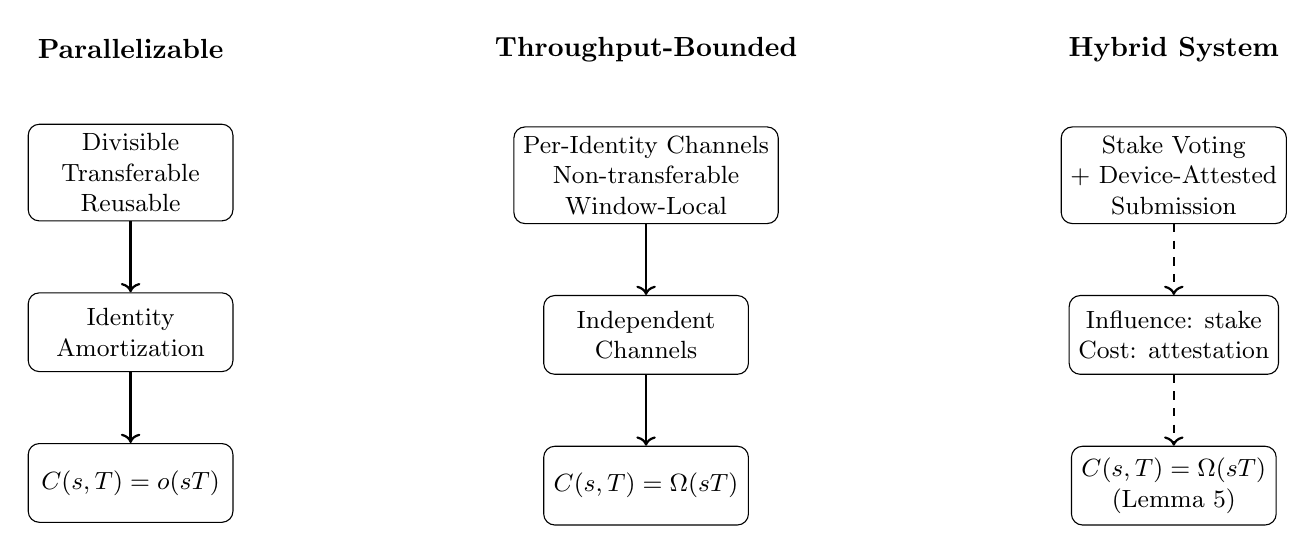
\begin{tikzpicture}[
			node distance=0.9cm and 1.8cm,
			every node/.style={font=\small},
			title/.style={font=\bfseries},
			box/.style={
				draw,
				rounded corners,
				align=center,
				minimum width=2.6cm,
				minimum height=1.0cm
			},
			arrow/.style={->, thick},
			dasharrow/.style={->, thick, dashed}
			]
			
			% ---- Titles ----
			\node[title] (lefttitle) {Parallelizable};
			\node[title, right=3.2cm of lefttitle] (midtitle)
			{Throughput-Bounded};
			\node[title, right=3.2cm of midtitle] (hybridtitle)
			{Hybrid System};
			
			% ---- Left column ----
			\node[box, below=0.7cm of lefttitle] (p1)
			{Divisible \\ Transferable \\ Reusable};
			\node[box, below=0.9cm of p1] (p2)
			{Identity\\Amortization};
			\node[box, below=0.9cm of p2] (p3)
			{$C(s,T)=o(sT)$};
			
			% ---- Middle column ----
			\node[box, below=0.7cm of midtitle] (t1)
			{Per-Identity Channels \\ Non-transferable \\ Window-Local};
			\node[box, below=0.9cm of t1] (t2)
			{Independent\\Channels};
			\node[box, below=0.9cm of t2] (t3)
			{$C(s,T)=\Omega(sT)$};
			
			% ---- Right column ----
			\node[box, below=0.7cm of hybridtitle] (h1)
			{Stake Voting \\ $+$ Device-Attested \\ Submission};
			\node[box, below=0.9cm of h1] (h2)
			{Influence: stake\\Cost: attestation};
			\node[box, below=0.9cm of h2] (h3)
			{$C(s,T)=\Omega(sT)$\\(Lemma~5)};
			
			% ---- Left arrows ----
			\draw[arrow] (p1) -- (p2);
			\draw[arrow] (p2) -- (p3);
			
			% ---- Middle arrows ----
			\draw[arrow] (t1) -- (t2);
			\draw[arrow] (t2) -- (t3);
			
			% ---- Hybrid arrows ----
			\draw[dasharrow] (h1) -- (h2);
			\draw[dasharrow] (h2) -- (h3);
			
		\end{tikzpicture}
		
		\caption{Structural geometry of adversarial identity cost.
			Parallelizable resources (left) enable identity amortization
			and sublinear cost. Throughput-bounded resources (center)
			enforce independent per-identity channels and linear cost.
			A hybrid governance system (right) combines
			stake-weighted aggregate influence with device-attested
			proposal submission; by Lemma~5, under additive decomposition
			assumptions, the throughput-bounded component dominates
			and linear adversarial cost is preserved.}
		
		\label{fig:resource-geometry}
	\end{figure*}
	
	\subsection{Per-Actor Throughput Channels}
	
	Let $\mathcal{U}$ denote a set of independent actors.
	Each actor $u \in \mathcal{U}$ is associated with a
	real-time execution channel $\mathcal{C}_u$ through which
	resource output is generated.
	
	\begin{definition}[Per-Actor Throughput Channel]
		A channel $\mathcal{C}_u$ is throughput-bounded if there exists
		a constant $\tau > 0$ such that for every window $t$
		\[
		\text{rate}_t(\mathcal{C}_u) \le \tau .
		\]
	\end{definition}
	
	The quantity $\text{rate}_t(\mathcal{C}_u)$ represents the maximum
	resource output attributable to actor $u$ during window $t$.
	Resource allocation for identity $v$ is derived from the channel output:
	
	\[
	r_v(t) \le \text{rate}_t(\mathcal{C}_u).
	\]
	
	This abstraction naturally induces throughput boundedness,
	identity non-transferability, and window-local temporal scope.
	Critically, it enforces that each identity must be backed by
	an independent execution channel, preventing cross-identity
	resource reuse.
	
	\subsection{Formal Classification}
	
	\begin{theorem}[Per-Actor Channel Classification]
		
		Let $R$ be a resource derived from per-actor throughput channels.
		Then $R$ satisfies (1) throughput boundedness,
		(2) failure of identity transferability,
		and (3) window-local temporal scope.
		Consequently $R$ belongs to the throughput-bounded
		non-parallelizable class.
		
	\end{theorem}
	
	\begin{proof}
		
		Throughput boundedness follows from the existence of the
		per-channel rate limit $\tau$.
		Identity transferability fails because resource generation
		is bound to the actor controlling channel $\mathcal{C}_u$.
		Window locality holds since each window requires fresh
		channel output. Thus the resource satisfies the defining
		properties of throughput-bounded non-parallelizable resources.
		
	\end{proof}
	
	\subsection{Examples of Throughput-Bounded Channels}
	Several real-world mechanisms naturally instantiate
	per-actor throughput channels.
	
	\paragraph{Human Real-Time Participation}
	Human participation constitutes one concrete realization
	of a throughput-bounded channel. Human cognitive processing,
	attention span, and motor interaction impose intrinsic limits
	on sustained activity. These physiological constraints bound
	the amount of verifiable activity a single actor can produce
	per time window. Increasing computational infrastructure
	does not increase the throughput of a human-bound channel.
	Thus adversarial scaling requires recruiting additional
	independent actors, making identity amplification
	economically linear in $s$.
	
	\paragraph{Device-Bound Execution}
	Hardware-bound environments can also induce throughput limits.
	Trusted execution environments, secure hardware tokens, and
	device attestation systems bind activity to physical
	hardware~\cite{costan2016intel}. Each device can produce
	only limited verifiable output within a time window.
	An adversary cannot reuse a single device to sustain multiple
	identities within the same window, preventing cross-identity
	amortization.
	
	\paragraph{Rate-Limited Network Participation}
	Not all rate-limiting mechanisms instantiate throughput-bounded
	resources in the sense of this paper. Ordinary account-level
	rate limits do not qualify unless they are structurally bound
	to non-transferable actors, devices, or execution channels.
	If identities can be created cheaply and limits are attached
	only to syntactic account identifiers, adversaries may bypass
	such constraints through identity replication.
	
	Throughput-boundedness therefore requires that rate constraints
	be tied to independent participation channels that cannot be
	aggregated or reassigned. Concrete examples include
	device-attested proposal submission, where each proposal must
	originate from a distinct attested hardware token, and
	hardware-rooted governance participation, where voting
	actions are bound to non-transferable execution environments.
	When such structural binding exists, per-identity execution
	constraints enforce adversarial cost that scales linearly
	with the number of identities.
	
	\subsection{Automation and AI}
	Automation does not invalidate the linear lower bound
	unless it eliminates the underlying throughput constraint.
	If participation requires independent channels whose
	throughput cannot be aggregated or transferred, scaling
	the number of identities still requires provisioning
	additional independent channels. The lower bound therefore
	depends on the persistence of actor-bound throughput
	constraints, not on assumptions about human uniqueness.
	
	\subsection{Hybrid Resource Models}
	
	Real-world systems rarely rely on a single security resource
	in isolation. Instead, deployed protocols often combine
	parallelizable and throughput-bounded resources. For example,
	a governance protocol may allocate voting power proportionally
	to financial stake while limiting proposal submission through
	per-identity rate constraints.
	
	\begin{lemma}[Hybrid Scaling Behavior]
		
		Let $R = (R_p, R_t)$ where $R_p$ is parallelizable
		and $R_t$ is throughput-bounded and non-transferable.
		If adversarial cost decomposes as
		
		\[
		C(s,T) = C_p(s,T) + C_t(s,T),
		\]
		
		then
		
		\[
		C_p(s,T) = o(sT), \qquad
		C_t(s,T) = \Omega(sT).
		\]
		
		Consequently
		
		\[
		C(s,T) = \Omega(sT).
		\]
		
	\end{lemma}
	
	\begin{proof}
		
		We consider the adversary's cost minimization problem
		under the hybrid resource $R = (R_p, R_t)$.
		
		\textbf{Step 1: Additive decomposition assumption.}
		We consider hybrid systems in which the total adversarial
		cost decomposes additively as
		\[
		C(s,T) = C_p(s,T) + C_t(s,T),
		\]
		representing independent resource constraints that contribute
		separably to adversarial expenditure.
		
		\textbf{Step 2: Bounding each component.}
		By Theorem~1, $C_p(s,T) = o(sT)$ since $R_p$ is
		parallelizable and admits identity amortization.
		By Theorem~2, $C_t(s,T) \geq c \cdot sT$ for some
		constant $c > 0$, since $R_t$ is throughput-bounded,
		non-transferable, and window-local.
		
		\textbf{Step 3: The throughput-bounded component dominates.}
		Since $C_t(s,T) = \Omega(sT)$ and $C_p(s,T) = o(sT)$,
		for sufficiently large $s$ the throughput-bounded term
		dominates:
		\[
		C(s,T) = C_p(s,T) + C_t(s,T) \geq C_t(s,T) \geq c \cdot sT.
		\]
		
		Therefore $C(s,T) = \Omega(sT)$.
		
	\end{proof}
	
	This result applies to additive decompositions of hybrid resources
	and should be interpreted as a sufficient structural characterization,
	rather than a complete description of all hybrid compositions.
	Non-additive hybrid compositions, in which the two resource
	components interact or partially substitute for one another,
	are outside the scope of this paper and remain an open
	direction for future work.
	
	Thus, throughput-bounded components act as a bottleneck
	that neutralizes identity amplification attacks enabled by
	parallelizable resources.
	
	\subsection{Analytical Illustration of the Scaling Laws}
	
	To illustrate the asymptotic bounds proved in
	Theorems~1--3 we consider closed-form expressions
	derived directly from the theoretical analysis.
	These curves are illustrative rather than empirical;
	they visualize the theoretical scaling behavior
	established in Theorems~1 and~2.
	
	For parallelizable resources the adversary incurs a fixed
	aggregate allocation cost
	\[
	C_p(s,T) = r_{\text{fixed}},
	\]
	while throughput-bounded resources require per-identity
	resource expenditure
	\[
	C_t(s,T) = r_{\min} \cdot s \cdot T .
	\]
	Figure~\ref{fig:theorem-validation} plots these expressions
	for $s \in [1,10{,}000]$ with $T=100$ windows.
	The parallelizable cost curve is flat, reflecting identity
	amortization and vanishing marginal identity cost.
	In contrast, the throughput-bounded curve grows linearly,
	confirming the asymptotic lower bound
	$C(s,T)=\Omega(sT)$.
	
	\begin{figure*}[t]
		\centering
		
\includegraphics[width=0.95\textwidth]{fig2_theorem_validation.pdf}
		
		\caption{Adversarial cost geometry derived from Theorems~1--3.
			\emph{Left}: total adversarial cost $C(s,T)$
			vs.\ sustained identities~$s$;
			parallelizable resources exhibit cost growing only
			with~$s$ (stock acquisition) whereas throughput-bounded
			resources enforce linear growth in both $s$ and~$T$.
			The crossover $s^{*} = r_{\mathrm{fixed}}/(r_{\min}T)$
			marks where throughput-bounded cost exceeds the
			parallelizable baseline.
			\emph{Right}: normalized total cost $C(s,T)/sT$;
			the parallelizable ratio declines as $s,T\to\infty$
			jointly (Theorem~1), while the throughput-bounded
			ratio remains bounded away from zero at $r_{\min}$
			(Theorem~2).
			Note that $C(s,T)/sT$ measures amortized cost per
			identity per window and should not be confused with
			marginal identity cost $\Delta(s,T) = C(s,T)-C(s-1,T)$,
			which for throughput-bounded resources satisfies
			$\Delta(s,T) \ge r_{\min}T$.}
		
		
		\label{fig:theorem-validation}
	\end{figure*}
	
	\subsection{Practical Enforcement of Throughput Bounds}
	
	The theoretical results developed in this paper assume the
	existence of non-transferable per-identity throughput bounds.
	In practice such constraints are approximated through
	mechanisms that bind resource generation to independent
	actors, devices, or execution environments.
	
	Examples include rate-limited protocol participation,
	device-attested computation, and human-interaction tasks.
	While no practical mechanism perfectly enforces strict
	non-transferability, systems that approximate these structural
	properties inherit the linear adversarial cost guarantees
	established in this work and effectively prevent identity
	amplification.
	
	% ============================================================
	\section{Adversarial Implications and Attack Surfaces}
	
	The asymptotic separation of Sections~V--VII has direct
	adversarial implications.
	When a resource is divisible and reusable, adversarial influence
	may be redistributed across identities while preserving aggregate
	capacity, enabling attacks that remain invisible under
	aggregate-weight security models.
	The key shift is from \emph{how much resource an adversary controls}
	to \emph{how adversarial cost scales as identities proliferate}.
	
	\subsection{Canonical Amortization Attack}
	
	Let $R$ be a divisible, reusable resource.
	An adversary: (i)~acquires aggregate allocation $r = s\,r_{\min}$;
	(ii)~partitions $r$ across $s$ identities (divisibility);
	(iii)~reassigns allocations via transferability; and
	(iv)~reuses allocations across windows (temporal reusability).
	By Lemmas~1--3, total cost satisfies
	\[
	C(s,T) \le s\,r_{\min} + h(s,T) = o(sT),
	\]
	so marginal cost $\Delta(s,T) = O(1) = o(T)$.
	The adversary expands the identity set without per-window renewal
	overhead---in contrast to rate-limited resources, where
	$\Delta(s,T) = \Omega(T)$.
	
	\subsection{Instantiation in Blockchain Systems}
	
	\paragraph{Proof-of-Work.}
	PoW is a hybrid.
	Mining \emph{capacity} (hardware) is divisible and transferable;
	mining pools implement identity partitioning by distributing hash
	power while maintaining aggregate control.
	Theorem~1 applies to this capacity component.
	\emph{Operational expenditure} (energy) is non-reusable and
	window-local, contributing a flow cost not captured by the
	divisible classification.
	The full economic cost of sustaining multiple mining identities
	combines both components.
	
	\paragraph{Proof-of-Stake.}
	Financial stake satisfies all four divisibility properties.
	Delegation markets enable a fixed capital base to be distributed
	across arbitrarily many validators.
	Under the considered model, stake therefore admits identity
	amortization: $C(s,T) = o(sT)$ with respect to the stake
	component.
	
	\subsection{Case Study: Stake-Governed Protocol}
	
	Consider a governance protocol where voting influence is
	proportional to delegated stake, proposal submission is
	rate-limited to one per identity per epoch, and committee
	membership is determined by per-identity sortition.
	
	\textbf{Attack.}
	An adversary controlling $1\%$ of total stake $S$ splits
	across $s = 100$ accounts, each holding $0.01S/100$.
	Total voting weight remains $0.01S$; proposal bandwidth
	expands to $100$ proposals per epoch.
	Since stake redistribution incurs no additional $T$-scaling
	expenditure, this amplification is essentially free under the
	considered model.
	
	\textbf{Structural analysis.}
	The stake component admits amortization by Theorem~1.
	If the rate limit is bound to non-transferable execution
	channels (e.g., device attestation), then by Theorem~2
	the participation component enforces $C_t(s,T) = \Omega(sT)$,
	and by Lemma~5 total cost satisfies $C(s,T) = \Omega(sT)$.
	If the rate limit is enforced only at the account level,
	without structural binding, the constraint is bypassable and
	the system reduces to the divisible regime of Theorem~1.
	
	\textbf{Design implication.}
	Identity-level security in hybrid protocols depends not on
	rate limits alone, but on whether those limits are structurally
	bound to non-transferable participation channels.
	
	\subsection{Governance Attack Surface}
	
	In identity-sensitive governance, an adversary controlling
	total stake $R$ may distribute it across $s$ identities without
	changing total voting weight, yet gain:
	increased proposal capacity, biased committee selection,
	amplified visibility in deliberation, and influence over
	rate-limited participation.
	These effects arise without increasing aggregate resource
	ownership and are not captured by classical aggregate-weight
	analyses.
	
	\subsection{Mitigation and Design Principle}
	
	Under the considered model, introducing per-identity
	throughput constraints bound to non-transferable channels
	may restore $C(s,T) = \Omega(sT)$.
	This suggests treating identity-level security as a co-design
	problem between protocol rules and resource structure.
	Systems that rely exclusively on divisible, reusable resources
	may admit amortization properties under the considered model; incorporating at least one rate-limited, non-transferable component appears necessary to resist identity amplification within this framework.
	
	Examples of such components include:
	actor-bound participation constraints,
	device-attested execution,
	non-transferable throughput tokens,
	or interaction channels requiring independent execution.
	\section{Limitations and Open Problems}
	
	While the structural separation established in this work
	identifies asymptotic constraints on adversarial identity scaling within the present model,
	several limitations and open questions remain.
	
	\subsection{Measurement of Throughput Constraints}
	
	Our analysis assumes the existence of a per-identity throughput bound
	$\tau$ and an activation threshold $r_{\min}$.
	In practice, accurately measuring and enforcing such constraints
	may be challenging.
	
	Real-world systems must ensure that throughput limits cannot be
	bypassed through aggregation, outsourcing, or hardware replication.
	If the effective per-identity throughput increases with additional
	infrastructure or automation, the linear lower bound may weaken.
	
	Designing robust mechanisms that enforce non-transferable,
	rate-limited participation therefore remains an important
	engineering challenge.
	
	\subsection{Verification and Measurement Overhead}
	
	Even when throughput-bounded resources exist,
	systems must verify that resource usage actually corresponds
	to independent identities or actors.
	
	Verification mechanisms---such as device attestation,
	interaction verification, or behavioral validation---
	may introduce additional complexity,
	latency, or economic cost.
	The present model excludes verification cost from $C(s,T)$;
	in practice, such costs may be non-negligible and should be
	incorporated into any concrete deployment analysis.
	
	Understanding the trade-offs between strong throughput
	verification and system scalability
	remains an open systems-design problem.
	
	\subsection{Coordinated Multi-Actor Adversaries}
	
	The lower bound shows that sustaining $s$ identities requires
	$\Omega(sT)$ resource expenditure when each identity must be
	supported by an independent throughput channel.
	
	However, adversaries may coordinate large numbers of actors.
	While such coordination does not violate the linear bound,
	it raises additional questions regarding economic feasibility,
	incentive compatibility, and the potential emergence of
	identity markets or participation outsourcing.
	
	Analyzing equilibrium behavior under large-scale coordinated
	participation remains an important direction for future work.
	
	\subsection{Hybrid Resource Models}
	
	Many real-world systems combine multiple resource classes,
	such as capital, computational effort, and human participation.
	
	Our separation theorem applies cleanly to pure resource classes,
	but hybrid constructions may exhibit intermediate scaling behavior.
	For example, systems that combine stake-weighted influence
	with rate-limited participation may simultaneously exhibit
	parallelizable and throughput-bounded properties.
	
	Partial results for additive hybrid compositions are established
	in Lemma~5 and Section~VIII-E, where the throughput-bounded
	component is shown to dominate asymptotically under additive
	cost decomposition. Characterizing adversarial scaling laws for
	non-additive hybrid compositions and more general resource
	interactions remains an open theoretical problem.
	
	\subsection{Adaptive and Evolving Resource Classes}
	
	Technological evolution may alter the structural properties
	of resources over time.
	For example, advances in automation or AI-driven participation
	may increase effective throughput or reduce non-transferability.
	
	Our framework provides a structural lens for analyzing such changes,
	but the validity of resource assumptions must be periodically
	reassessed as system environments evolve.
	
	\subsection{Beyond Linear Scaling}
	
	This work distinguishes between sublinear and linear
	identity-scaling regimes.
	Other scaling geometries---such as superlinear or convex
	adversarial cost growth---may arise under stronger
	structural constraints.
	
	Identifying minimal structural conditions that enforce
	stronger-than-linear identity cost remains an open
	theoretical direction.
	
	\subsection{Protocol-Level Realization}
	
	The results of this paper are structural and protocol-agnostic.
	Translating these guarantees into deployable systems
	requires careful engineering of verification mechanisms,
	incentive compatibility, and liveness properties.
	
	Bridging the structural theory of security resources
	with fully composable distributed implementations
	remains a promising avenue for future research.
	
	\subsection{Adaptive Economic Incentives and Governance Dynamics}
	
	The present framework models adversarial cost as a deterministic
	function of resource allocation, abstracting away adaptive
	economic behavior, endogenous governance dynamics,
	and evolving participation incentives.
	In practice, sustained identity cost may be influenced by
	market prices for delegated resources, token inflation,
	regulatory changes, and governance rules that adjust thresholds
	in response to observed participation patterns.
	The framework intentionally isolates structural resource
	properties rather than modeling complete governance ecosystems.
	Incorporating adaptive incentive structures and endogenous
	governance dynamics remains an important direction for future work.
	
	\subsection{Automation and Evolving Throughput}
	
	The linear lower bound for rate-limited resources rests on the
	assumption that per-identity throughput constraints are enforced
	and cannot be circumvented by additional infrastructure.
	Advances in automation, AI-driven participation, and hardware
	acceleration may progressively reduce the effective cost of
	provisioning independent execution channels, potentially narrowing
	the practical gap between the two scaling regimes even when the
	theoretical separation holds asymptotically.
	The framework provides a structural lens for analyzing such
	changes, but the validity of throughput assumptions should be
	periodically reassessed as deployment environments evolve.
	
	\subsection{Socio-Economic Behaviors and Identity Markets}
	
	The model treats adversarial identity creation as a direct
	resource acquisition problem, abstracting away socio-economic
	coordination mechanisms.
	In practice, identity markets, participation outsourcing,
	and secondary markets for rate-limited credentials may alter
	the effective cost structure in ways not captured by the
	abstraction, potentially weakening non-transferability assumptions
	in practice even when they hold structurally.
	Analyzing equilibrium behavior in such settings remains outside
	the scope of the present work.
	
	\subsection{Scope of the Framework}
	
	The results developed in this paper characterize adversarial
	identity scaling under an abstract structural model.
	The framework is not intended as a complete empirical taxonomy
	of deployed systems, nor does it claim that all real-world
	systems can be perfectly classified into purely divisible or
	rate-limited categories.
	Rather, it isolates structural properties that govern asymptotic
	scaling behavior under explicit assumptions, providing a
	complementary perspective alongside deployment-specific and
	protocol-level analyses.
	Real deployments may exhibit partial transferability,
	imperfect throughput enforcement, or hybrid resource composition;
	in such settings, the scaling geometry may interpolate between
	the regimes characterized here.
	
	\subsection{Window Size and Temporal Granularity}
	
	The system model partitions time into discrete windows
	of uniform size, and the adversarial cost function
	$C(s,T)$ is defined over a horizon of $T$ such windows.
	The choice of window size is therefore a modeling parameter
	that affects how the results apply to concrete systems.
	
	Smaller windows correspond to finer temporal granularity,
	increasing the number of renewal events required for
	sustained participation under throughput-bounded resources.
	In the limit of very small windows, the per-window
	activation cost $r_{\min}$ may approach zero while $T$
	grows proportionally, leaving the product $r_{\min} \cdot T$
	roughly constant. The linear lower bound
	$C(s,T) \geq r_{\min} \cdot sT$ therefore remains
	meaningful provided that $r_{\min}$ and $T$ are
	calibrated consistently with the chosen window granularity.
	
	Larger windows reduce the number of renewal events
	but may allow adversaries to concentrate resource
	expenditure within a single window, potentially
	relaxing the window-locality constraint.
	Systems in which resource allocation persists across
	multiple windows should be modeled with correspondingly
	larger $r_{\min}$ or reduced effective $T$.
	
	More generally, the window size assumption interacts
	with the throughput bound $\tau$ and the activation
	threshold $r_{\min}$ in ways that depend on the
	deployment context. Characterizing the sensitivity
	of the scaling bounds to window granularity---and
	identifying window-size-independent formulations
	of the structural separation---remains an open
	direction for future work.
	
	% ============================================================
	\section{Analytical Illustrations of Scaling Regimes}
	\label{sec:evaluation}
	
	We visualize the cost functions implied by Theorems~1 and~2
	under parametric variation.
	These are analytical illustrations of asymptotic scaling
	behavior derived from the theoretical model---not
	empirical benchmarks or experimental proofs.
	
	\subsection{Setup}
	
	We evaluate the model cost functions directly:
	$C_{\mathrm{par}}(s,T) = s \cdot r_{\min} + h(s,T)$
	for divisible resources (one-time stock acquisition plus
	coordination overhead), and
	$C_{\mathrm{bnd}}(s,T) = s \cdot T \cdot r_{\min}$
	for rate-limited resources (mandatory per-identity,
	per-window expenditure).
	Throughout, $r_{\min} = 1.0$.
	For E4, three coordination models are tested:
	$h_1 = s + T$, $h_2 = s\log T$, $h_3 = s\sqrt{T}$,
	all satisfying $h(s,T) = o(sT)$.
	
	\subsection{E1: Identity Scaling ($T=100$, vary $s$)}
	
	The normalized cost $C_{\mathrm{par}}(s,T)/sT$ decreases
	monotonically from $1.02$ at $s=1$ to $0.03$ at $s=100$,
	consistent with $C(s,T)=o(sT)$ (Theorem~1).
	The rate-limited ratio remains at $1.0$ for all $s$,
	consistent with $C(s,T)=\Theta(sT)$ (Theorem~2).
	
	\begin{table}[!htbp]
		\centering
		\small
		\caption{E1: Normalized adversarial cost $C(s,T)/sT$
			($T=100$, $r_{\min}=1.0$, $h = s+T$).}
		\label{tab:e1}
		\renewcommand{\arraystretch}{1.2}
		\begin{tabular}{@{}rrrrr@{}}
			\toprule
			$s$ & $C_{\mathrm{par}}$ & $C_{\mathrm{par}}/sT$
			& $C_{\mathrm{bnd}}$ & $C_{\mathrm{bnd}}/sT$ \\
			\midrule
			1   & 102.0  & 1.0200 & 100.0   & 1.0000 \\
			5   & 110.0  & 0.2200 & 500.0   & 1.0000 \\
			10  & 120.0  & 0.1200 & 1000.0  & 1.0000 \\
			25  & 150.0  & 0.0600 & 2500.0  & 1.0000 \\
			50  & 200.0  & 0.0400 & 5000.0  & 1.0000 \\
			100 & 300.0  & 0.0300 & 10000.0 & 1.0000 \\
			\bottomrule
		\end{tabular}
	\end{table}
	
	\begin{figure}[!htbp]
		\centering
		
\includegraphics[width=\columnwidth]{fig_e1_identity_scaling.pdf}
		\caption{E1: Normalized adversarial cost $C(s,T)/sT$
			vs.\ $s$ ($T=100$).
			Divisible-resource ratio decays toward zero
			(Theorem~1); rate-limited ratio is constant at
			$r_{\min}$ (Theorem~2).}
		\label{fig:e1}
	\end{figure}
	
	\subsection{E2: Time Horizon Scaling ($s=10$, vary $T$)}
	
	$C_{\mathrm{par}}$ grows as $O(s+T)$, well below $sT$,
	while $C_{\mathrm{bnd}}$ tracks $sT r_{\min}$ exactly.
	The normalized divisible ratio continues to decrease as $T$
	grows, consistent with Theorem~1.
	
	\begin{table}[!htbp]
		\centering
		\small
		\caption{E2: Normalized cost $C(s,T)/sT$
			($s=10$, $r_{\min}=1.0$, $h = s+T$).}
		\label{tab:e2}
		\renewcommand{\arraystretch}{1.2}
		\begin{tabular}{@{}rrrrr@{}}
			\toprule
			$T$ & $C_{\mathrm{par}}$ & $C_{\mathrm{par}}/sT$
			& $C_{\mathrm{bnd}}$ & $C_{\mathrm{bnd}}/sT$ \\
			\midrule
			10  & 30.0   & 0.3000 & 100.0  & 1.0000 \\
			25  & 45.0   & 0.1800 & 250.0  & 1.0000 \\
			50  & 70.0   & 0.1400 & 500.0  & 1.0000 \\
			100 & 120.0  & 0.1200 & 1000.0 & 1.0000 \\
			150 & 170.0  & 0.1133 & 1500.0 & 1.0000 \\
			200 & 220.0  & 0.1100 & 2000.0 & 1.0000 \\
			\bottomrule
		\end{tabular}
	\end{table}
	
	\begin{figure}[!htbp]
		\centering
		
\includegraphics[width=\columnwidth]{fig_e2_time_scaling.pdf}
		\caption{E2: $C(s,T)$ vs.\ $T$ ($s=10$).
			Divisible cost grows sublinearly; rate-limited
			cost is linear in $T$ (Theorems~1--2).}
		\label{fig:e2}
	\end{figure}
	
	\subsection{E3: Marginal Identity Cost ($T=100$)}
	
	$\Delta_{\mathrm{par}}(s,T) = O(1)$ for all $s$;
	$\Delta_{\mathrm{bnd}}(s,T) = T \cdot r_{\min} = 100$
	throughout.
	The latter is consistent with the lower bound
	$\liminf_{s\to\infty}\Delta(s,T) \ge r_{\min} T$
	established in Theorem~2.
	
	\begin{figure}[!htbp]
		\centering
		
\includegraphics[width=\columnwidth]{fig_e3_marginal_cost.pdf}
		\caption{E3: Marginal cost $\Delta(s,T)$ vs.\ $s$
			($T=100$).
			Rate-limited: $\Delta = T \cdot r_{\min} = 100$
			(Theorem~2 lower bound, dashed).
			Divisible: $\Delta = O(1) = o(T)$ (Theorem~1).}
		\label{fig:e3}
	\end{figure}
	
	\subsection{E4: Coordination Overhead Robustness ($T=100$)}
	
	All three models yield $C_{\mathrm{par}}(s,T)/sT \to 0$,
	well below the rate-limited baseline of $1.0$.
	The sublinear regime is robust across the class $h(s,T)=o(sT)$,
	consistent with Assumption~\ref{ass:coordination}.
	
	\begin{table}[!htbp]
		\centering
		\small
		\caption{E4: $C_{\mathrm{par}}(s,T)/sT$ under three
			overhead models ($T=100$, $r_{\min}=1.0$).}
		\label{tab:e4}
		\renewcommand{\arraystretch}{1.2}
		\begin{tabular}{@{}rrrrr@{}}
			\toprule
			$s$ & $h_1{=}s{+}T$ & $h_2{=}s\log T$
			& $h_3{=}s\sqrt{T}$ & Bounded \\
			\midrule
			1   & 1.0200 & 0.0562 & 0.1100 & 1.0000 \\
			5   & 0.2200 & 0.0562 & 0.1100 & 1.0000 \\
			10  & 0.1200 & 0.0562 & 0.1100 & 1.0000 \\
			25  & 0.0600 & 0.0562 & 0.1100 & 1.0000 \\
			50  & 0.0400 & 0.0562 & 0.1100 & 1.0000 \\
			100 & 0.0300 & 0.0562 & 0.1100 & 1.0000 \\
			\bottomrule
		\end{tabular}
	\end{table}
	
	\begin{figure}[!htbp]
		\centering
		
\includegraphics[width=\columnwidth]{fig_e4_coordination.pdf}
		\caption{E4: $C_{\mathrm{par}}(s,T)/sT$ under three
			overhead models, all satisfying $h=o(sT)$.
			All decay toward zero (Theorem~1); rate-limited
			baseline (solid) remains at $r_{\min}$ (Theorem~2).}
		\label{fig:e4}
	\end{figure}
	
	\smallskip
	\noindent
	Illustrations E1--E4 are drawn from the theoretical cost
	functions and do not constitute experimental evidence about
	deployed systems.
	They confirm that both scaling regimes are consistent across
	the model parameter space, and that the marginal cost bound
	of Theorem~2 is tight.
	% ============================================================
	\section{Conclusion}
	
	This paper proposed an axiomatic framework for reasoning about
	adversarial identity scaling in open systems through the lens
	of resource structure.
	The central contribution is not a universally complete
	characterization of Sybil resistance, but a resource-centric
	asymptotic perspective that complements existing protocol-level
	and economic analyses.
	
	We formalized resource properties---divisibility, additivity of
	influence, temporal reusability, identity transferability, and
	throughput boundedness---and showed that these properties indicate
	the asymptotic geometry of sustained adversarial cost under the
	coordination model considered.
	Within the present abstraction, resources satisfying divisibility
	and reusability admit identity amortization, suggesting a
	structural tendency toward sublinear per-identity cost.
	Conversely, rate-limited, non-transferable, window-local resources
	indicate the scaling regime $C(s,T)=\Omega(sT)$.
	
	Analytical illustrations confirmed that these two scaling regimes
	are consistent across varying identity counts, time horizons, and
	coordination overhead models within the framework, and that the
	marginal cost bound associated with rate-limited resources is tight.
	These illustrations are drawn from the theoretical cost functions
	and do not constitute experimental evidence about deployed systems.
	
	Taken together, these results suggest an asymptotic boundary
	in the design space of open systems.
	Under the assumptions considered, mechanisms grounded in fully
	divisible and reusable resources may be insufficient to enforce
	linear per-identity cost under the considered assumptions.
	Security guarantees at the identity layer are therefore
	constrained not only by aggregate resource scarcity,
	but by the structural properties of the resource used to
	regulate participation.
	
	This perspective is intended as a complement to, rather than a
	replacement of, existing security analyses.
	Classical consensus models and economic equilibrium analyses
	capture important adversarial dimensions outside the scope of
	this work.
	The framework here isolates a different dimension: the degree to
	which resource divisibility and reusability enable adversarial
	cost amortization across identities and time.
	
	Future work includes characterization of hybrid resource
	compositions, mechanisms for enforcing practical throughput bounds,
	analysis of equilibrium behavior under adaptive economic incentives,
	and empirical measurement of identity-scaling behavior in live
	open systems.
	% ============================================================
	\appendices
	
	% ============================================================
	\section{Tightness and Robustness of the Scaling Bounds}
	% ============================================================
	
	This appendix establishes that the asymptotic bounds derived in
	Theorems~1 and~2 are tight and remain robust under several
	extensions of the adversarial model.
	
	In particular, we construct explicit adversarial strategies that
	match the asymptotic upper and lower bounds associated with the
	two structural resource classes introduced in this work.
	These constructions demonstrate that the separation between
	sublinear and linear identity-scaling regimes is not merely
	qualitative, but asymptotically exact.
	
	% ============================================================
	\subsection{Tightness for Parallelizable Resources}
	
	Let $R$ be a parallelizable resource satisfying divisibility,
	additivity of influence, temporal reusability, and identity
	transferability.
	
	By the activation threshold (Definition~1), sustaining $s$
	identities requires aggregate allocation at least
	$r \ge s\,r_{\min}$.
	For a parallelizable resource the adversary acquires this
	aggregate \emph{once}: by temporal reusability, the allocation
	$r = s\,r_{\min}$ suffices for all $T$ windows without
	renewed expenditure.
	
	By divisibility, the adversary partitions $r$ into components
	$r_1,\dots,r_s$ with $\sum_{i=1}^{s} r_i = r$.
	By additivity of influence,
	\[
	\sum_{i=1}^{s} f(r_i)
	=
	f\!\left(\sum_{i=1}^{s} r_i\right)
	=
	f(r).
	\]
	
	Hence total influence is invariant under identity partitioning.
	The total adversarial cost satisfies
	\[
	C(s,T) \le s\,r_{\min} + h(s,T).
	\]
	
	Under Assumption~1, $h(s,T)=o(sT)$. Therefore
	\[
	\frac{C(s,T)}{sT}
	\le
	\frac{r_{\min}}{T}
	+
	\frac{h(s,T)}{sT}
	\to 0
	\qquad \text{as } s,T \to \infty \text{ jointly},
	\]
	since the first term vanishes as $T\to\infty$ and the
	second by assumption.
	
	Thus $C(s,T)=o(sT)$, confirming that the sublinear
	scaling regime of Theorem~1 is asymptotically tight.
	
	
	% ============================================================
	\subsection{Tightness for Throughput-Bounded Resources}
	% ============================================================
	
	Let $R$ be a throughput-bounded resource satisfying
	Definition~6, with activation threshold $r_{\min}$
	and window-local allocation.
	
	Consider an adversary sustaining $s$ identities over
	$T$ windows.
	
	By construction, each identity must receive at least
	$r_{\min}$ units of resource within every active window.
	Allocating
	\[
	r_v(t)=r_{\min}
	\]
	for all identities $v$ and windows $t$ yields total cost
	\[
	C(s,T)
	=
	\sum_{t=1}^{T}
	\sum_{v=1}^{s}
	r_{\min}.
	\]
	
	Evaluating the sum gives
	\[
	C(s,T)=sT r_{\min}.
	\]
	
	Therefore,
	\[
	C(s,T)=\Theta(sT),
	\]
	which matches the lower bound established in Theorem~2.
	
	Hence the linear scaling regime is also asymptotically tight.
	
	\medskip
	\noindent
	Together, these constructions establish that the two asymptotic
	regimes identified in this paper represent tight structural
	characterizations of adversarial identity scaling.
	
	% ============================================================
	\section{Robustness Under Extended Adversarial Models}
	% ============================================================
	
	We now examine the robustness of the scaling results under
	natural extensions of the adversarial model.
	
	The objective is not to characterize every possible adversarial
	behavior, but to demonstrate that the structural separation
	remains stable under several realistic variations.
	
	% ============================================================
	\subsection{Adaptive Identity Creation}
	% ============================================================
	
	Suppose the adversary creates identities adaptively over time.
	
	Under parallelizable resources, adaptive creation does not alter
	the scaling regime, since aggregate resource ownership may still
	be repartitioned across newly created identities.
	
	Under throughput-bounded resources, each newly activated identity
	must continue to satisfy the per-window activation threshold.
	Therefore adaptive creation preserves the lower bound
	\[
	C(s,T)=\Omega(sT).
	\]
	
	% ============================================================
	\subsection{Coalitions of Independent Actors}
	% ============================================================
	
	Suppose an adversary coordinates $k$ independent actors, each
	associated with a throughput-bounded execution channel.
	
	Although aggregate throughput increases with $k$, sustaining
	$s$ concurrent identities still requires at least $s$
	independent channels.
	
	Thus coalition formation does not invalidate the linear lower
	bound, and
	\[
	C(s,T)=\Omega(sT)
	\]
	continues to hold.
	
	% ============================================================
	\subsection{Stochastic Throughput Bounds}
	% ============================================================
	
	Consider a setting in which throughput is stochastic but bounded
	in expectation.
	
	Let $\tau_v(t)$ denote the random throughput available to
	identity $v$ during window $t$, with bounded expectation
	\[
	\mathbb{E}[\tau_v(t)] \le \tau.
	\]
	
	If sustained participation requires expected activation
	threshold $r_{\min}$ per identity per window, then expected
	total expenditure satisfies
	\[
	\mathbb{E}[C(s,T)] = \Omega(sT).
	\]
	
	Under standard concentration assumptions, deviations from the
	expected cost remain bounded with high probability, preserving
	linear scaling asymptotically.
	
	% ============================================================
	\subsection{Partial Relaxation of Structural Properties}
	% ============================================================
	
	The framework developed in this paper characterizes two
	extremal structural regimes: fully parallelizable resources
	and fully throughput-bounded resources.
	
	Intermediate systems may partially satisfy transferability,
	temporal locality, or throughput boundedness.
	In such cases, adversarial scaling behavior may interpolate
	between the asymptotic regimes established in Theorems~1--2.
	
	For example, if only a fraction of aggregate allocation is
	transferable across identities, the adversary may amortize
	only that component of the resource.
	Likewise, bounded temporal reuse across a limited number of
	windows may reduce, but not eliminate, sustained expenditure.
	
	These intermediate cases suggest a continuum of scaling
	behaviors between sublinear amortization and linear growth.
	
	Formal characterization of such transition regimes, including
	potential phase boundaries between amortizable and
	non-amortizable resources, remains an important direction
	for future work.
	
	
	% ============================================================
	\bibliographystyle{IEEEtran}
	\bibliography{references}
	% ============================================================
	
\end{document}